
%(BEGIN_QUESTION)
% Copyright 2010, Tony R. Kuphaldt, released under the Creative Commons Attribution License (v 1.0)
% This means you may do almost anything with this work of mine, so long as you give me proper credit

The flow rate of a fluid measured by a {\it counterpropagation} (``transit-time'') ultrasonic flowmeter is given by the following formula:

$$Q = k {t_{up} - t_{down} \over (t_{up})(t_{down})}$$

$$\includegraphics[width=15.5cm]{i03522x01.eps}$$

Knowing that the time for a sound wave to propagation upstream is equal to the length of the travel path divided by the difference in sound wave and fluid velocities ($t_{up} = {L \over {c - v}}$) and that the time for a sound wave to propagation downstream is equal to the length of the travel path divided by the sum of sound wave and fluid velocities ($t_{down} = {L \over {c + v}}$), prove that the flow rate measurement ($Q$) does not depend on the speed of sound through the fluid ($c$).  In other words, substitute these mathematical definitions for $t_{up}$ and $t_{down}$ into the flowmeter equation and simplify to show that $c$ is eliminated (canceled out) in the end.

\vfil 

\underbar{file i03522}
\eject
%(END_QUESTION)





%(BEGIN_ANSWER)

This is a graded question -- no answers or hints given!
 
%(END_ANSWER)





%(BEGIN_NOTES)

The trickiest portions of this manipulation are combining fractions with unlike denominators.  Recall from arithmetic that we need the denominators of two or more fractions to be identical before we may add the numerators together (e.g. $3 \over 5$ + $1 \over 4$ cannot be directly added until we find a lowest common denominator and then modify the fractions accordingly: ${12 \over 20} + {5 \over 20} = {17 \over 20}$).  In the case of literal expressions rather than numerical expressions, we may obtain a common denominator simply by multiplying the two unlike denominators (e.g. ${x \over y} + {a \over b} = {bx \over by} + {ay \over by} = {bx + ay \over by}$).

$$Q = k {t_{up} - t_{down} \over (t_{up})(t_{down})}$$

$$Q = k {{L \over {c-v}} - {L \over {c+v}} \over \left({L \over {c-v}}\right) \left({L \over {c+v}}\right)}$$

$$Q = k {{L (c+v) \over {c^2-v^2}} - {L (c-v) \over {c^2-v^2}} \over {L^2 \over {c^2-v^2}}}$$

$$Q = k {{{L (c+v) - L (c-v)} \over {c^2-v^2}} \over {L^2 \over {c^2-v^2}}}$$

$$Q = k \left({{L [(c+v) - (c-v)]} \over {c^2-v^2}}\right) \left({{c^2-v^2} \over L^2}\right)$$

$$Q = k {{(c+v) - (c-v)} \over L}$$

$$Q = k {2v \over L}$$

$$Q = {2kv \over L}$$

Note how $c$ is nowhere to be found!  This tells us it is irrelevant to the measurement of flow.  The only variables affecting our flow measurement are fluid velocity ($v$), path length ($L$), and the ``fudge factor'' $k$ accounting for the angle between path length and flow axis among other things.

%INDEX% Mathematics review: manipulating literal equations

%(END_NOTES)


